\myChapter{Service Oriented Architecture: technologies and restrictions for designing services for EAs}\label{chap:soa} %cuidado con
                                %los títulos. Si estás hablando de
                                %algoritmos evolutivos también, tienes
                                %que mencionarlo en el título, porque
                                %si quien lo lea ya sabe de SOA se lo
                                %salta - JJ %FERGU: Mejor este título? (para distinguirlo del siguiente)

%PREGUNTAS PARA JJ:
% ¿Está bien el título de este capítulo?
% Mencionar metodologías? (SOMA y todas esas)

\minitoc\mtcskip
\vfill
\lettrine{T}{he} previous chapter has explained some shortcomings % some
                                % lacks? algunas faltas? something
                                % lacking no es lo mismo que some
                                % lacks y no se debe usar en este
                                % contexto formal - JJ FERGU: cambiado a shortcomings en este y otros capis
 in the development of EAs, mainly related with the integration of
 different frameworks, distributed programming and heterogeneity of
 computational environments, among others. This chapter explains the
 concept \textsc{Service Oriented Architecture} (SOA), with several
 associated technologies and methodologies, as a possible solution for
 these issues. %Tienes que tener siempre mucho cuidado con qué
               %consideras parte de la tesis o no. Esto NO lo es pero
               %por la introducción parecía que ibas a introducir una
               %solución que no existía en el estado del
               %arte. Recuerda que tienes siempre que tener claro el
               %mapa mental de dónde encaja cada pieza dentro de la
               %TESIS y aquí no lo estás dejando. Y ten claro que la
               %tesis es TU tesis, no un review de SOA - JJ

Research in SOA \cite{Papazoglou2007SOA} is a growing field, % si
                                % el artículo es de 2007 yo diría que
                                % ya ha terminado de emerger. - JJ FERGU: cambiado a growing (sigue creciendo, pero no emerge)
as can be seen in Figure \ref{fig:soapapers}, obtained from the search
terms {\em ``service oriented OR service-oriented''} in the Scopus
\footnote{\url{http://www.scopus.com}} database. Each year more papers
about the topic are published. This area seeks to promote services
usage and adoption, and to improve the way to use them. For example,
solving a problem combining existing services in an automatic way
\cite{Moussa2010ServiceComposition}. % Proponer una metodología
                                % porque se publica mucho equivale a
                                % decir que la vas a dejar si no se
                                % publica tanto. Es muy
                                % tricky. Deberías de pensar en algún
                                % otro mérito - JJ FERGU: puesto a continuación que se usa mucho también en la empresa. Ya, ya, no es el mundo académico, pero podemos decir que así están más unidos.
Not only in the academic world, but also in the industry, with more than an 
seventy percent of adoption and satisfaction \cite{Heffner10strong}, adding significant value to the enterprises \cite{Heffner13soa}.

% En la conclusión del capítulo anterior has dicho que este capítulo iba a resolver diferentes asuntos. ¿Qué asuntos está resolviendo? ¿Qué propones, en general y en particular, para resolverlos? - JJ FERGU: Escrito al final de la introducción para resumir lo que vamos a resolver



\begin{SCfigure}[20][tb]
\centering
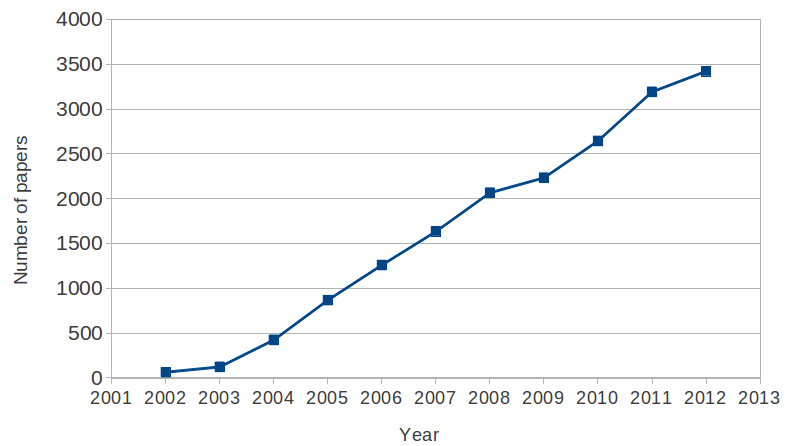
\includegraphics[width=26pc]{gfx/soa/papersYear.png}
\caption{Number of published papers (per year) about SOA (obtained from Scopus database).}
\label{fig:soapapers}
\end{SCfigure}


Service Oriented Architecture (SOA) is a computational
paradigm where agents % users o applications? o agents? - JJ FERGU: cambiado a agents, que es lo más genérico
interact with each other using loosely coupled, coarse-grained, and autonomous components called 
{\em services} \cite{rotem2012soa}. A service is a distributed entity (such as a node, program or
function), used to obtain a result, increasing the integration of heterogeneous
systems (several operating systems, protocols or languages) due to
this multi-platform nature. The service users do not need to know
the language used to implement the service, and they are not
forced to use a specific technology to access that service. For
example, an evolutionary algorithms researcher could have access to a
fitness function made publicly available by another researcher at the
other side of the world without even knowing which programming language
has been used to implement it. % podrías decir la relación que tiene
                               % esto con la ciencia abierta,
                               % resultados reproducibles y demás - JJ - FERGU: lo explico adelante

Also, with the advancement of the Internet, new scientific
communities, based on interoperable and distributed platforms are
emerging. These communities allow scientist to collaborate on their
research, sharing data and remote access to their programs. To achieve
this, they use SOA, obtaining the benefits of the standards it
offers. Users publish and use flexible, interoperable and configurable
services. These services can be created from scratch or by leveraging
existing software \cite{Bechhofer2013ResearchObject}. % un ejemplo!!! - JJ FERGU: esta frase es tuya del paper de la SoCo xD (ejemplo puesto)

\person{Foster} \cite{Foster2005Science} defines the term ``Service Oriented
Science'' as the pursuit of scientific research using distributed and
interoperable networks, being the uniformity of
these interfaces the key to success. Thanks to it, researchers can discover and access
the services without developing specific access for each data source, or
program. %ejemplos!! - JJ FERGU: abajo
Therefore, this paradigm has the potential to increase the
scientific productivity due to these public and distributed services,
and also to increase the data analysis automation in computing. There
are many examples that attempt to boost this paradigm, like Open
Science Grid \cite{Altunay2011OpenScience} and GLOBUS
\cite{Foster2005Globus}.  %citep o cite? - JJ FERGU: era de un paper mío, cambiado
These projects include scientific communities and globally distributed infrastructures that support scientific and integrated applications of different domains.

It is necessary to remark that the technology for implementing services is not the
key challenge in SOA, but to increase the effort to migrate the
existing work and to change the mind of researchers and
practitioners. This is, therefore, one of the aims of this thesis: to  
present to EA researchers the benefits of adopting this paradigm, describing the SOA concepts,
restrictions and methodologies, but also to present the most
used technologies to chose the most adequate one.
%to what? Esto relaciónalo con la tesis, es un capítulo
               %de TU TESIS - JJ FERGU: añadido "one of the aims of this thesis..." y también lo de abajo

In this chapter, the usage of SOA is proposed to facilitate the shortcomings in the EAs presented in the previous chapter: development, integration, standardization and dynamism. First, several concepts to undarsted SOA are explained. Then the most used technologies and methodologies are presented and how can help with the previous shortcomings. After that, the benefits of using SOA in EAs are explained, but also the restrictions of SOA are listed in order to be considered when creating a methodology to develop evolutionary algorithms in this paradigm. 


\section{What is a Service?}
\label{sec:soa:whatis}
\lettrine{A}{} service can be seen as a function call which can be
executed locally or remotely, and which is independent of the
programming language or running platform. As previously said, services have well defined
interfaces, which depends on the desired technology to implement
SOA. That means that the service users do not need to know the
language implementation of the service or the operating system, %esto
                                %ya lo has dicho - JJ FERGU: pongo el "as previously said" lo pongo, pero para que quede claro y se le meta al lector en la cabeza
 and they are not forced to use a specific technology to access to that service.






Figure \ref{fig:soadiagram} shows the basic interaction among
services. First, the \textsc{service provider} exposes the service, publishing
its interface in the \textsc{service broker}. The \textsc{service consumer} (or
\textsc{requestor}) finds  a service in the broker to be used and receives its
interface. Then the request is performed by the \textsc{consumer} (which uses or
consumes the service).  

\begin{SCfigure}[20][tb]
\centering
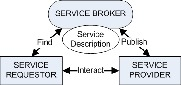
\includegraphics[width=20pc]{gfx/soa/soaDiagram.jpg}
\caption{Service interaction schema. The service provider publishes a
  service description that is used by the consumer to find and use the
  service.} % no has definido consumer todavía - JJ FERGU: movida la imagen de sitio para definirlo antes
\label{fig:soadiagram}
\end{SCfigure}



According to \person{Valipour} \cite{Valipour09surveysoa}, services to develop must follow these characteristics:

\begin{itemize}
\item {\em Discoverable and Dynamically Bound}: Services must be discoverable. Thanks to the service registry, a service consumer can discover a service to be use at runtime.
\item {\em Self-Contained and Modular}: All functions in SOA are services. This means that every
  component in SOA must be modelled as a service, or as an aggregation of services. The services are well-defined: the interface of the service must be fixed, and it can not change in time, because the consumers or implementations of this interface should be modified with it. Services are, therefore, {\em encapsulated}: only the interface should be used to consume a service.
\item {\em Interoperability}: Consumers do not need to know how the service implementation performs their function, as services behave as a ``black box''. This is, elements such as the programming language or distribution protocol are independent.
\item {\em Loose Coupling}: Services should be designed to need only a few number of well-known dependencies.
\item {\em Location Transparency}: Services must be indistinguishably local or remote, being independent of the protocol to establish the connection.
\item {\em Composability}: Developing applications in SOA means to aggregate different existing services. Services are designed to be {\em re-usable}.
\end{itemize}



Moreover, several implementations of a specific service  can exist (in
one or several machines). The broker can choose which one to use  each
time, or offer another if a service is temporarily
unavailable. Implementations  may also have a different behaviour, so
the researcher can take advantage to create an auto-adaptive algorithm
to select different implementations according to some criteria. % esto
                                % tenías que haberlo hecho para la
                                % tesis!!! - jj FERGU: Experimento realizado y puesto en capítulos siguintes
Figure \ref{fig:servicebasic} shows this special interaction, where two different implementations of an operator interface exist (even using different languages) and the broker has chosen one of them.


The service broker in a SOA can be implemented in several ways and have
different behaviours: for example, the implementations of the services to be used can be
defined in a text file (if the services do not change in execution
time). However, the broker can also assign implementations to
interfaces in an automatic way, or using several rules. For example, in the context of EAs,
to select a better operator if the current one is not working properly.
%to distribute a fitness between several machines activated while the
%algorithm is running. % ¿vas a hacerlo? ¿No? Trata de restringirte a
                      % lo que vas a hacer en la tesis, porque si no
                      % te preguntarán que por qué diablos no lo has
                      % hecho - JJ FERGU: cambiada la frase


\begin{SCfigure}[20][tb]
\centering
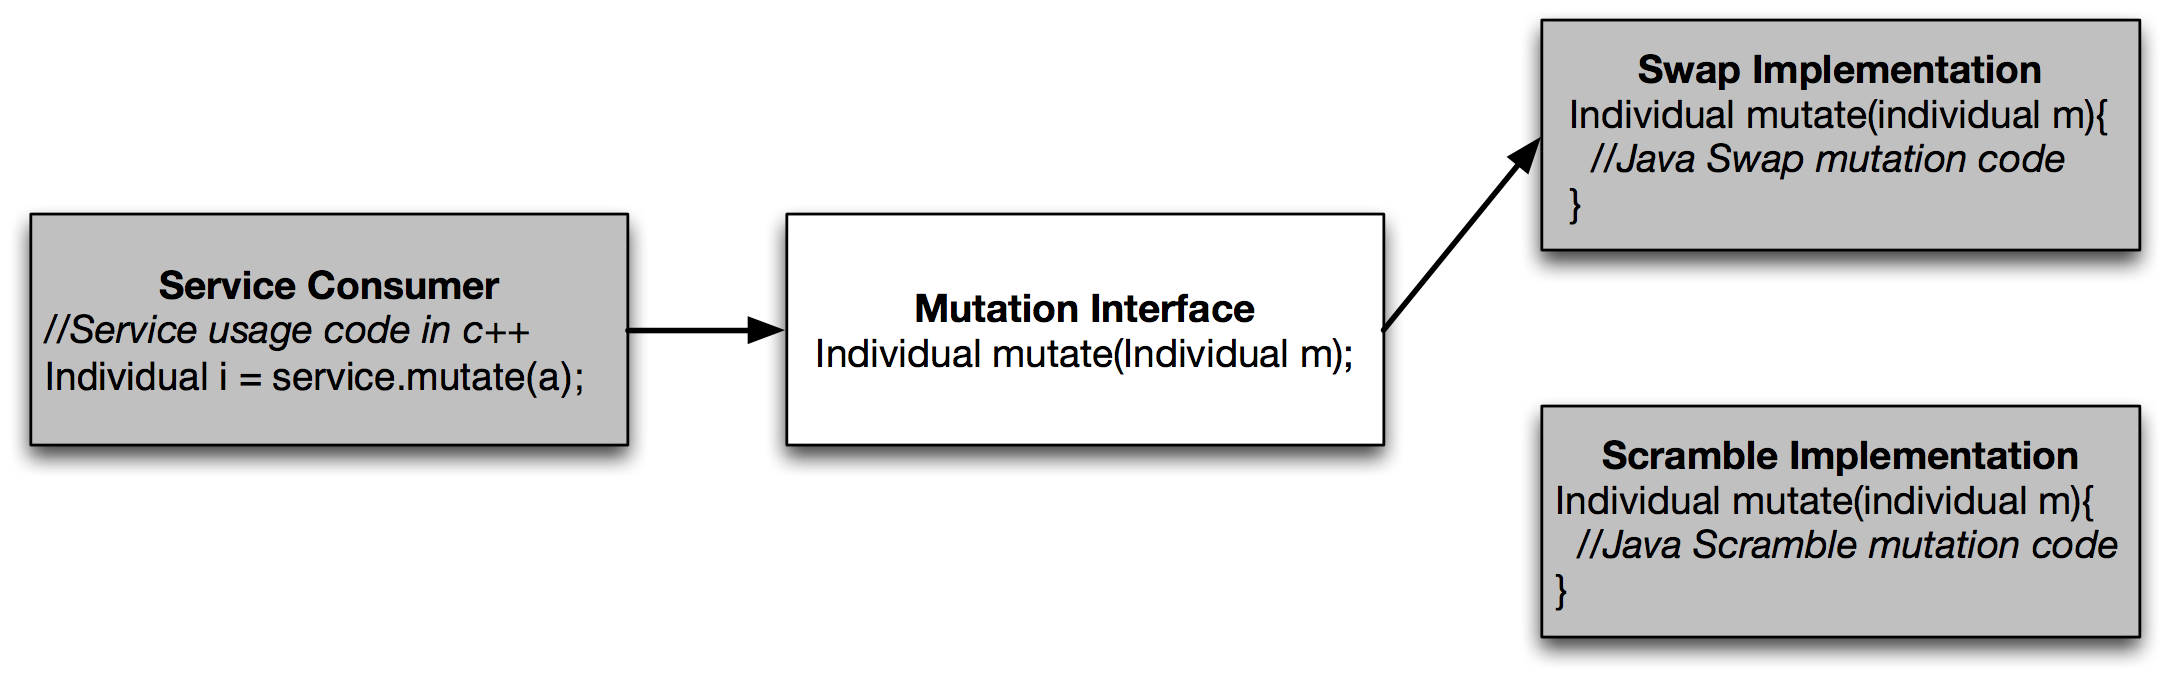
\includegraphics[width=26pc]{gfx/soa/exampleSOA.jpg}
\caption{Example of usage of a service implementation.}
\label{fig:servicebasic}
\end{SCfigure}




An important SOA capability is that it is not focused on a specific
implementation, but offers a set of guidelines to help the
developers. In \cite{Arsanjani2008SOMA} these guidelines and good practices, and also the differences between SOA and Object Oriented
Programming (OOP) are
explained: the main difference between SOA and imperative programming or OOP is the order of service execution. This order is not necessarily static, because the services are designed to be used in a non-established and configurable order. Furthermore, another important difference is that services can be dynamically discovered and used (while in OOP a function/method must be previously known and can not change during execution), being also one of the most important capabilities the (optional) distribution in a network. Finally, in OOP the programming language must be the same for each method call.

\section{Implementation technologies}
\label{chap:soa:implementations}

\lettrine{D}{espite} the fact that the concept of service is independent of the technology used, there exist several ways to use and implement services, being Web Services, REST, \definicion{ebXML}{Electronic Business XML} and \definicion{OSGi}{Open Service Gateway Initiative} the most extended.

\subsection{Web Services}
\label{subsec:soa:ws}
One of most popular services implementations are  \textsc{Web
  Services} \cite{Papazoglou2007SOA}. A web service is a service that
is available over Internet that uses any standardized XML (eXtended
Meta Language) \cite{XML} messaging system, and it is not tied to any
specific language or operating system \cite{Cerami2002Webservices}.
As SOA proposes, web services should be self-describing (using a
standardized grammar) and self-discoverable. % secciones de un párrafo
                                % no son secciones - JJ FERGU: No, lo de abajo es sub-sub-section, no tiene numeración, pero el resaltado queda bien.

\subsubsection{Messaging system} There are several alternatives to the messaging system, as SOAP or XML-RPC. SOAP (Simple Object Access Protocol) is a standard protocol proposed by the W3C \cite{SOAP}  which  extends the XML remote procedure call (XML-RPC) standard. 
It is a complete and mature protocol that allows performing remote
method calls to distributed routines (services) based on an XML
interface. % SOAP se usa cada vez menos me parece a mi. Podías
           % indicarlo. - JJ FERGU: Cierto, SOAP se está usando menos en web, pero en la empresa. Lo pongo al hablar de REST 

SOAP clients can access objects and methods that are residing in
remote servers, using a standard mechanism that makes  the details of
implementation transparent, such as the programming language of the
routines, the operating system or the platform used by the provider of
the service. % esto lo has repetido por enésima vez - JJ
At the moment, there exist complete implementations of SOAP for Perl, Java, Python, C++ and most modern languages.
Unlike other remote procedure call methods, such as RMI (Remote method invocation, used by the Java language) or XML-RPC, SOAP has two main advantages: it can be used with any programming language, and it can use any type of transport (\definicion{HTTP}{HyperText Transfer Protocol}, \definicion{TCP}{Transmission Control Protocol}, \definicion{SMTP}{Simple Mail Transfer Protocol} and other protocols). In this way, SOAP constitutes a high level protocol, making easy the task of distributing objects among different servers, and avoiding the difficulties derived of defining the message formats, nor the explicit call to remote servers.


\subsubsection{Self-description} The interfaces of the methods of web services that can be accessed are specified by a Web Services Description Language (WSDL) \cite{WSDL}. The WSDL of a web service consists in an XML description of its interface, i.e., it is a file that describes the name of the methods, their parameters (number and type) and their type of response.

\subsubsection{Self-discovery} UDDI ({\em Universal Description, Discovery and Integration}) \cite{UDDI} is a technical specification for describing, discovering and integrating web services \cite{Cerami2002Webservices}. This specification includes APIs for the storage and retrieval of information (also in an standardized XML format).


\subsubsection{Other standardizations} One of the advantages of using
web services % nunca coma entre sujeto y predicado - JJ FERGU: OK
 is that the application stack is growing with the WS-Extensions. That is, the basic specifications of Web Services (such as SOAP) can be extended with transactions, security or messaging, for example. The most used are \cite{Papazoglou2007SOA}:
\begin{itemize}
  \item WS-Addressing  (authentication)
  \item WS-Security , WS-SecureConversation  and WS-Trust  (authorization and secure messaging)
  \item WS-Policy and WS-Metadata Exchange (policy mechanisms for interactions)
  \item WS-Reliable Messaging  and WS-Transaction (add-on mechanisms for the communication channel)
\end{itemize}
% pero todo esto importa lo más mínimo para la tesis? Lo vas a usar? FERGU: explicado después
% No metas rollo por meterlo - JJ
Also, functional extensions, such as WSRF \cite{WSRF}, % qué
                                % significa? - JJ
 allows the discovery, inspection and interaction with stateful resources in standard and interoperable ways. Finally, BPEL ({\em Business Process Execution Language})  \cite{BPEL} is an XML-based language to control the invocation of different Web services with added business logic to help large-scale programming.

The main advantage of using Web Services in research is their public discovering and usage, thanks to the security extensions. Several studies about e-science taking advantage of web services can be found in bibliography \cite{Oinn04Taverna,davidson08workflows,Ludascher06Kepler,Perera06workflows}.

\subsection{REST}
\textsc{Representational State Transfer} (REST)\footnote{\url{http://en.wikipedia.org/wiki/Representational_state_transfer}} is an alternative method to build web services.
This architectural style % no es una tecnología, es una convención!!! - JJ FERGU: cambiado a architectural style
was proposed and defined by \person{Fielding} in \cite{Fielding2002}.

In a REST-style architecture, a client sends requests to the server, who processes them and returns responses to the client.
Requests and responses represent resources that can be addressed by a Uniform resource identifier (URI). Usually, resources are documents or programs the client need to access.

REST usually works over the HTTP protocol. However it can be based on other protocols that provide the appropriate mechanisms to send requests and return responses.

In a REST environment, while servers are not concerned with the client state, clients only take about their own state and how to address resources on the server using URIs. Moreover, clients can cache responses to improve performance.
As the client-server communication is stateless, servers are simpler and more scalable. 
Taking this into account, if the REST interface is not altered, servers and clients can be modified independently.
Finally, servers can customize the functionality of the clients by sending their logic (code) to be executed.


REST web services are simple and lightweight (as no extra XML markup
is needed), their message format is readable by humans, they are easy
to build, and finally, developments achieve a high performance
\cite{Daigneau2011}. % podías citar el trabajo de Pedro SOAP vs. REST
                     % - JJ
The main differentiating factor is that Web Services using SOAP tend to be operation-based, while REST services are resource-based. This is one of the reasons REST is replacing SOAP on the web \cite{Mason11REST}. %FERGU: puesto lo de que se usa menos en la web

\subsection{ebXML}
ebXML defines a set of standards that allows the enterprises negotiate their products through the Internet. It is based on a well-defined documents interchange using a contract-based approach \cite{Patil03ebxmlVsWS}, providing a specification for messaging, registry/repositories and business processes description, and unlike other approaches, it is an horizontal standard (it is not oriented towards a specific industry sector). On the contrary, Web Services expose any kind of applications to the Web, so anyone can call them (service approach). Another significant difference between Web Services and ebXML is that the former is based on BPEL, which can only describe the scenario inside a company, due to it has not all the information about the services being orchestrated, while the latter can be used to model a global choreography among several companies. Due to this, and because it is mainly focused to commercial and business processes, this technology is not going to be addressed in this thesis.

\subsection{OSGi}
\label{subsec:soa:osgi}
OSGi was proposed by a consortium of more than
eighty companies in order to develop an infrastructure for the
deployment of services in heterogeneous network of devices, mainly
oriented to domotics \cite{GarciaSanchez2013Gateway}. Nowadays it defines a
specification for a SOA for virtual
machines (VMs). It provides very desirable features, like
packet abstraction, life-cycle management, packaging or versioning, % qué significa todo esto? - JJ FERGU: Añado ref
allowing a significant reduction of the building, support and deployment
complexity of the applications. These features can be useful in the field of EAs, as suggested by \person{Wagner \etal} \cite{WagnerPlugins07}.

OSGi technology allows dynamic discovery of new components (or services), to increase the collaboration and to minimize and manage the coupling
among modules. Moreover, the
OSGi Alliance has developed several standard component interfaces for
common usage patterns, like HTTP servers, configuration, logs, security,
management or XML management among others, whose implementations can
be obtained by third-parties. %Nowadays there are some challenges
% nowadays y citas un trabajo del 2008? - JJ
%in the OSGi development \cite{Kriens2008OsgiChallenges}, but they only
%affect the creation of very complex applications. % y, como dicen en
                                % mi pueblo, los algoritmos evolutivos
                                % son más simples que paja de habas? - JJ
                                %FERGU: meh, lo comento todo, tampoco era muy interesante

These advantages are not so
                               costly as can be thought: on one hand the OSGi
                                framework can be implemented in a
                                {\em jar} file\footnote{A jar file is
                                a file that groups some compiled Java
                                files.} of about 300KB, and on the other hand, and differing from
                                the normal usage of Java, each
                                class pre-charges only the other
                                classes it needs, not all. Also it is
                                non-intrusive: the code to be
                                executed in OSGi can be executed
                                without it. Finally, from its
                                specification in 1998 has been widely
                                used as base in big projects: the
                                Eclipse \definicion{IDE}{Integrated Development
                                Environment} is built over OSGi, and
                                also big application servers
                               (Glassfish\footnote{\url{http://glassfish.java.net}} 
                               or IBM Websphere \footnote{\url{http://www.ibm.com/software/websphere/}}) or
                               residential gateways
                               \cite{GarciaSanchez2013Gateway}, among other
                               examples. 



%\subsubsection{Distribution}
In OSGi all services can be distributed using the OSGi
features, simply setting which service is distributable and which is
the distribution technology that provides service discovering and data
transmission.   % so what? - JJ % ¿Esto es relevante? - JJ FERGU: TODO sí, esto es MUY relevante, lo uso en la tesis, pero antes es que era una sección más grande. Pregunta: menciono aquí que  voy a usar OSGi en mi tesis o en el capítulo Osgiliath? (ahora está en ese capítulo)

\section{Methodologies for developing SOA}
\label{chap:soa:methodologies}
\lettrine{R}{egardless} of the chosen SOA framework, the processes % business? no estamos hablando de algoritmos - JJ FERGU: sí, es que a veces se les llama así, pero lo quito para no liar
 of the platform must be analysed and modelled. So it is necessary to use a consistent and well-defined methodology to design a model based on a machine-readable description \cite{Garcia09UMM}. {\em Business-Centric Methodology (BCM) for Enterprise Agility and Interoperability} \cite{Oasis03BCM} is a roadmap for the development and implementation of procedures to create effective, efficient, and sustainable interoperability mechanisms. It has been developed by OASIS, the same consortium that created BPEL or UDDI, among others, and it is complementary to other existing architectures and technologies designed to build business oriented services, like ebXML or Web Services. BCM is formed by a set of model layers with a step-guide process, and an information pyramid to align the semantic information of partners. This allows the participation of business experts and the creation of a very large documentation repository. Nevertheless, this methodology has some disadvantages: it has a very large learning curve and it is not very extended yet. 



{\em \definicion{UN/CEFACTs}{United Nations Center for Trade
    Facilitation and Electronic Business} Modelling Methodology (UMM)}
\cite{Hofreiter06UMM} is an approach to model the business services
that each partner must provide in order to perform a
\definicion{B2B}{Business to Business} collaboration. It has a
complete meta-model about business processes and business information,
including a process analysis methodology. It is interesting to show
that UMM provides and supports components to capture the knowledge
about the business processes, and that it is independent of the
underlying implementation technology (ebXML, Web Services,
\definicion{CORBA}{Common Object Request Broker Architecture} or
\definicion{EDI}{Electronic data interchange}). Furthermore, because
UMM extends \definicion{UML}{Universal Modelling Language}, we could
say that this methodology is more easily adaptable, due to the high
development, acceptance and maturity of UML \cite{Garcia09UMM}. In
fact, a survey of B2B modelling languages show that UMM is the most
complete approach \cite{Folmer08b2b}. 

Finally, {\em SOMA} (Service Oriented Modelling and Architecture)
\cite{Arsanjani2008SOMA} is an architecture proposed by IBM to model
service oriented processes. It lets the identification, specification
and implementation of  the services, flows and components inside the SOA paradigm. To achieve
this tasks, it proposes a top-down modelling oriented to
intra-enterprise services (service-oriented instead of
business-oriented). It is more agile than the previous ones
and it is not focused in enterprise environments. 

%Pero ¿esto lo vas a usar? ¿Le interesa lo más
                    %mínimo al revisor y/o tribunal? - JJ FERGU: si, cambiado el capitulo siguiente




%%%%%%%%%%%%%%BENEFICIOS DE USAR SOA EN EAs
\section{Benefits of using SOA in Evolutionary Algorithms Area}
\label{sec:soa:benefitsofsoa}

\lettrine{S}{OA} has been previously used in the EA area. For example,
web services have been used in the grid area for optimization
problems, as can be seen in the works of
\cite{grid1,grid2,grid3,grid5}, where services are defined using WSDL
interfaces and other transmission mechanisms (such as Remote Procedure
Call \cite{grid6,grid7}). Although EAs are executed in grids
\cite{grid8,grid4,grid10}) no information about how to design these
services for EAs has been provided in previous works.  % estás
                                % diciendo que no hay una metodología
                                % para diseñar estos servicios y eso
                                % es gordo, porque entonces tienes que
                                % hacerlo tú - JJ FERGU: Hecha la metodología en el capítulo siguiente :)

In the previous chapter several shortcomings % y dale - JJ FERGU: cambiado a shortcomings
 in the Evolutionary Algorithms area were presented, such as the new trends of
 distributed programming where nodes enter and exit in runtime, or the
 incompatibility between frameworks, for example. All these facts
 motivate the creation of a proper way to define services for evolutionary algorithms. The elements that combine an EA are candidate to be designed as services, as they can behave as input/output functions. Also, SOA solve the problems previously addressed: 



\begin{itemize}
\item {\em Development}: there exist several methodologies to model and design services. Also, as services are re-usable, they can be combined in different ways to create the different types of EAs. Moreover, existing technologies, also facilitate the development, using techniques such as versioning, packaging or life-cycle control.
\item {\em Integration}: Services are independent of the programming language. For example, services implemented in Java may use services implemented in C++ and vice-versa. Also, services allow distribution transparency: it is not mandatory to use a specific library for the distribution, or modify the code to adapt the existing operators. Existing EA frameworks could also be adapted to be accessed as services, providing their interfaces. 
\item {\em Standardization}: Interfaces of services use public
  standards (such as WSDL \cite{WSDL} or OSGi \cite{OSGI}). The
  service interfaces for EAs should be abstract enough to avoid their
  modification. Furthermore, as \person{Foster} claims
  \cite{Foster2005Science}, SOA is the key to develop Open Science. 
\item {\em Dynamism}: Services are not aware of the order of execution, so this paradigm can fit with new parallel approaches for EAs, where the control of the nodes is not centralized. Also, SOA provides techniques for automatic discovering of services. For example, new operators in different nodes can be bound and used during the run of an algorithm. Also, there should be easy to add and remove elements to achieve self-adaptive mechanisms.
\end{itemize} 


% no te repitas. Eso ya lo has dicho
                        % antes. Suena a que estás metiendo morralla
                        % por rellenar - JJ FERGU: Borrado ENTERO y reescrito arriba. Tambíen borrado abajo otros párrafos que me repetía mucho

% vaya, aquí lo dices, pero antes no - JJ FERGU: (era lo de open science) sí, está dicho arriba (y citado)







%%%%%%%%%%%%%%%%%%%%%%RESTRICCIONES EN SOA PARA DISEÑAR EAs
\section{Restrictions in SOA design for EAs}
\label{sec:soa:restrictions}
To allow these benefits the services for EAs should match with the next technological
restrictions: % ¿por qué? ¡Justifícalo todo! - JJ FERGU: Cambiada la primera frase para justificar lo siguiente

\begin{itemize}
\item The services can be dynamically bound to change the needed EA aspects. %bind o be bound - JJ FERGU: arreglado
\item The source code of  the basic EA services should not be  re-written or re-compiled to achieve this task. That means that the design must be as abstract as possible. % seriously? must not been? - JJ FERGU: arreglao
\item New services can be added in execution time. 
\item No specific source code for a distribution must added, neither  the existing source code of the services should be modified for this purpose (that is, changing distribution libraries must not add extra code in existing services). 
\end{itemize}


%In previous chapter we also presented the advantages of using SOA in Evolutionary Algorithms area: firstly, SOA fits with the genericity advantages in the development of software for EAs \cite{GENERICITY05} and adds new features, like language independence and  distribution mechanisms. It also allows the addition and removal of services in execution time without altering the general execution of the algorithm (that is, it is not mandatory to stop it or to add extra code to support new operators). This issue increases the interoperability between different software elements. Moreover, this allows easy code distribution: SOA does not require the use of a concrete implementation or library.
%FERGU: comentado este párrafo, que me repito (antes estaba en otro capítulo)






One of the main restrictions in SOA, % ¿SOA o SOAs? será "a SOA" o
                                % "SOAs", ¿no? - Jj FERGU: no, SOA es una metodología de diseño
 apart from focusing on the development of abstract services, is the
 stateless and un-ordered nature of services. Therefore, services must follow the next guidelines.
 % ¿Puede estar esto relacionado con
                                % programación funcional? Podías mirar
                                % y citar los papers de Albert al
                                % respecto - JJ FERGU: no, no está relacionado (pero ya cito los papers de Albert antes)

First, as services are unaware of each other, there should not be global
variables in any part of the code. Services are listening, and waiting
to be executed. For example, a fitness service with a counter that is
increased each time is called (to stop the algorithm if a limit is
reached, for example). If several (and different) algorithms were
working in parallel, and calling this function concurrently, the
counter could not distinguish between algorithms, giving erroneous
results. However, a service that maintains some kind of state is
allowed, for example, a statistics service that reads events from all
the algorithms being executed at the same time, but this should be
managed to avoid errors. % ¿en qué quedamos entonces? ¿Se permite o no
                         % se permite? - JJ

Also, a service should not be distinguishable from local or remote
running in other node in the network. % es la 5ª vez que dices esto - JJ FERGU: sí, pero ahora lo enlazo con los EAs
Every stage in the algorithm should be treated as a service to be
executed in local or in remote, even the {\em Population} or the {\em
  Parameters}. Mechanisms to ensure the correct data-sharing should be
provided. Also, many implementations of the same service could exist
at the same time (different implementations of {\em Crossover}, for
example) and it should be correctly managed and used. % pero ¿las va a
                                % haber? ¿Vas a usar estas
                                % características? - JJ FERGU: sí, las va a haber y lo voy a poner en el experimento (aunque estaba descrito en siguientes capítulos)

Moreover, a service is always a request-response function. For
example, the fitness calculation should not be a method of the {\em
  Individual} implementation, but a function that receives a list of
individuals and returns a list of the calculated fitness of that
individuals. This allow, for example, remote fitness calculation and
distributed load balancing, impossible to perform if the fitness is a
method of the {\em Individual} class. % Esto ya se hizo cuando
                                % diseñamos los Evolving Objects,
                                % podías citarlo - JJ FERGU: 

Thinking as abstract as possible requires to separate concepts such as
the order of recombination, and the crossover itself. Usually, after
parent selection, individuals are crossed in order. However, if we
need a different mechanism for mating (for example, using more than
two parents, or parent selected several times) a duplication of effort
is needed. That is the reason to separate the concept {\em
  recombine} from {\em crossover} (and also, following the top-down
design proposed in SOMA).  % ¿Esto es lo único que estás usando del
                           % SOMA? - JJ FERGU: no he cambiado el capítulo siguiente a saco

Finally, no assumptions should be taken about services previously
executed or being executed next. For example, the {\em Mutation} 
service could be applied before the {\em Recombination} or the fitness could be calculated in the middle of the generation. %For example, services to implement {\em
  %Recombinator} or {\em Mutator} should return the individuals with
%their fitness already calculated. % ¿Por qué? ¿Eso no implica que el
                                % mutador tiene que saber que existe
                                % otro servicio que calcula el
                                % fitness? Además, en la práctica el
                                % mutador no necesita el fitness (casi
                                % nunca)- JJ FERGU: cierto, quitado
Usually this step is performed in
the last stage of the generation, but if we require the individuals
for other tasks: for example, a Local Search or a statistics collector
to guide the algorithm. % if we require, ¿qué? - JJ FERGU: ejemplo puesto

\section{Conclusions}

\lettrine{E}{ven} as SOA is used extensively in software development area, it is
not widely accepted in the main EA software, as the survey of frameworks by \person{Parejo et al.}, presented in Section \ref{chap:distributed:conclusiones} claim. % pruébalo - JJ FERGU: Probado con la referencia al survey
The authors of these frameworks should improve their frameworks adding SOA technologies in
order to facilitate the communication and integration among them, without
 duplication of effort to re-program all the EA elements, and therefore, saving time. 
 Therefore, the benefits of using SOA in development, integration, standardization 
 and dynamism (presented in Section \ref{sec:soa:benefitsofsoa}) could be applied.
  % ¿y qué se conseguiría con eso? - JJ FERGU: reescrito y añadidas cosas
 Although all the approaches described Section \ref{sec:distributed:parallel} are focused
 on the implementation of distributed EAs, the abstraction level of
 each alternative can be quite different, as shown in Figure
 \ref{fig:soagrid}.  As SOA is a paradigm and not a technology,
 areas such as Evolutionary Robotics, or EA classic frameworks can use
 SOA to be designed and developed. Implementation technologies, such
 as Web Services, can fill the gap between SOA (abstract) and grid
 (infrastructure) where interfaces are designed using SOA principles
 (dynamism, visibility, loose-coupling and heterogeneity). Finally,
 cloud computing can be seen as a combination that extends SOA adding
 the scalability of the grid, ad suggested by \person{Jamil}
 \cite{SOALIB}. % y esto es interesante porque.. - JJ


\begin{SCfigure}[20][tb]
\centering
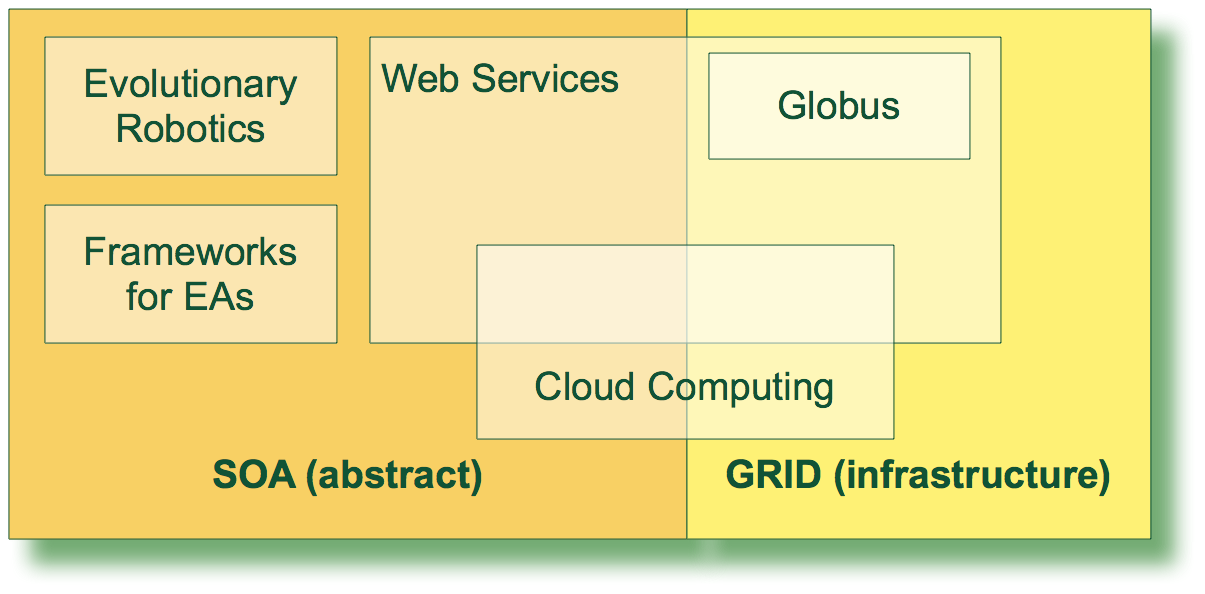
\includegraphics[width=26pc]{gfx/soa/soagrid.png}
\caption{SOA as abstract paradigm to develop EAs in different
  areas. %¿to develop qué? ¿o to be developed? - JJ FERGU: arreglado
 Using specific technologies such as Web Services allows grid integration. This figure has been updated from the one presented in \cite{SOALIB}.}
\label{fig:soagrid}
\end{SCfigure}
In this thesis the SOMA guidelines (identification, specification and
realization of the services, flows and components) are going to be used, because it is the
% Esto tienes que decirlo donde estés hablando de SOMA. - JJ FERGU: puesto
methodology more flexible and less focused on commercial
purposes. Next chapter will present a methodology to use the design principles of SOA for
developing services for EAs. Then, in later chapters, a specific SOA technology will be
used to develop an implementation of a service oriented architecture
for EAs.
